\section{Results and Evaluation}
\label{sec:evaluation}
This chapter will focus on the evaluation of the different subsystems of the project, and offer a critical analysis of the project as a whole. The evaluation will be based on the project's ability to meet the requirements set out in the project specification, as well as the project's performance in terms of accuracy, efficiency, and usability. The evaluation will also consider the limitations of the project and suggest areas for future work.

\subsection{Mechanical Design}

\subsection{Electronics and Software}

\subsection{Computer Vision}
\label{sec:computer-vision-evaluation}
This section will evaluate the Computer Vision system, as discussed in \autoref{sec:computer-vision-system} and implemented in \autoref{sec:computer-vision}.

\subsubsection{Component Detection Model}
The Component Detection model was trained on a dataset of 976 images, split into a 70-20-10 split for training, validation, and testing respectively. The dataset was augmented using the augmentations discussed in \autoref{sec:image-processing}. The model was trained using the training parameters shown in \autoref{tab:training-parameters}.

\begin{figure}[H]
    \centering
    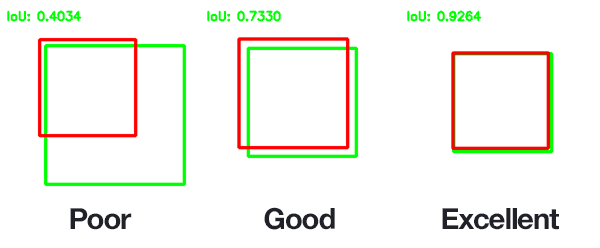
\includegraphics[width=0.8\textwidth]{imgs/articles/iou.png}
    \caption{IoU Example \cite{rosebrock_2016}}
    \label{fig:iou}
  \end{figure}
  
As discussed in \autoref{sec:real-time-object-detection}, mAP\raisebox{-1pt}{\textsuperscript{50}} is a standard metric used to evaluate object detection models. mAP\raisebox{-1pt}{\textsuperscript{50-95}} is a more rigorous metric that aggregates the mean average precision across all classes at different Intersection over Union (IoU) thresholds; in mAP\raisebox{-1pt}{\textsuperscript{50}}, an object is considered as detected if the IoU is greater than 0.5 (the predicted bounding box overlaps the ground truth bounding box by at least 50\%), whereas in mAP\raisebox{-1pt}{\textsuperscript{50-95}}, the mAP score is aggregated across different IoU thresholds from 0.5 to 0.95 in steps of 0.05. This can be seen more clearly \autoref{fig:iou}.
  
  \begin{figure}[H]
    \centering
    \includesvg[width=0.8\textwidth]{imgs/graphs/metrics_mAP50-95(B).svg} 
    \caption{TensorBoard graphing: all runs mAP\raisebox{-1pt}{\textsuperscript{50-95}} against epochs}
    \label{fig:metrics}
  \end{figure}
  
In \autoref{fig:metrics}, the mAP\raisebox{-1pt}{\textsuperscript{50-95}} is shown for all training runs of the model with slightly different training parameters. It can be seen that the models tend to converge around 20 epochs, and there is a ceiling at around 80\% mAP\raisebox{-1pt}{\textsuperscript{50-95}}. This is likely due to the small dataset size, and it is made even smaller due to the use of a test set. For deployment, the training set will absorb the test set to increase the size of the dataset and improve the model's performance, however for discussion it is necessary to keep a test set separate to evaluate the model's performance. 
  
  
  \todo{talk about tensor board}
  \todo{show metrics}
  
On the GTX 3080 Ti, 
  
Interestingly, if Class Loss is set to 1.0, Box Loss is set to 4.0, and DFL is set to 1.5, the model converges in around ~15 epochs, taking only ~2 minutes to train. However, the model's performance is slightly impacted, calculating metrics on the test set yields an mAP\raisebox{-1pt}{\textsuperscript{50-95}} of 77.8\%, but it was decided that the time savings were not worth it given it was only a few minutes of training time. The model was therefore trained with the parameters shown in \autoref{tab:training-parameters}.

\todo{show pictures of model in action}

\subsubsection{Resistor Value Classification Model}

\todo{add power consumption measurements from usb for complete power - implementation maybe?}
